%%% Preamble
% Article class of KOMA-script with 11pt font and a4 format
\documentclass[paper=a4, fontsize=11pt]{scrartcl}	
\usepackage[T1]{fontenc}
\usepackage{fourier}

% English language/hyphenation
\usepackage[english]{babel}

% Better typography
\usepackage[protrusion=true,expansion=true]{microtype}

% Math packages
\usepackage{amsmath,amsfonts,amsthm}

% Enable pdflatex
\usepackage[pdftex]{graphicx}
\usepackage{url}


%%% Custom sectioning (sectsty package)
% Custom sectioning (see below)
\usepackage{sectsty}
% Change font of al section commands
\allsectionsfont{\centering \normalfont\scshape}


%%% Custom headers/footers (fancyhdr package)
\usepackage{fancyhdr}
\pagestyle{fancyplain}

% No page header
\fancyhead{}

% You may remove/edit this line 
\fancyfoot[L]{\small SIGB Hand-in 1}
\fancyfoot[C]{} % Empty
\fancyfoot[R]{\thepage} % Pagenumbering
\renewcommand{\headrulewidth}{0pt} % Remove header underlines
\renewcommand{\footrulewidth}{0pt} % Remove footer underlines
\setlength{\headheight}{13.6pt}


%%% Equation and float numbering
\numberwithin{equation}{section} % Equationnumbering: section.eq#
\numberwithin{figure}{section} % Figurenumbering: section.fig#
\numberwithin{table}{section} % Tablenumbering: section.tab#


%%% Maketitle metadata
\newcommand{\horrule}[1]{\rule{\linewidth}{#1}} % Horizontal rule

\title{
		%\vspace{-1in} 	
		\usefont{OT1}{bch}{b}{n}
		\normalfont \normalsize \textsc{IT University of Copenhagen} \\ [25pt]
		\horrule{0.5pt} \\[0.4cm]
		\huge How Did We Build An Eye Tracker \\
		\horrule{2pt} \\[0.5cm]
}

\author{
	\normalfont 
	\normalsize
	Miroslav Zoricak, Jorge Castillo R.\\[-3pt]		
	\normalsize
	\today
}

\date{}


%%% Begin document
\begin{document}
\maketitle

\section{Introduction}

We were tasked with the construction of a software eye tracker. In the following text we describe our approach to this challenge, the methods we have used, and the results we have obtained.  We have built the eye tracker using Python and OpenCV as a toolkit. The purpose of the eye tracker is to correctly and accurately detect the eye (pupil, iris) and glints on the eye in every image where there is an eye and detect nothing if there is no eye present in the image.

In general, eye tracker algorithms are reducing a huge amount of data (typical 640x480 RGB image is almost 1MB of uncompressed data) to just a few values representing the location and radius of pupil, iris and various glints. Therefore there must be many ways of performing this reduction, some better than others. Our goal in this report is to describe the approach we have taken to solving this problem, which algorithms we have used and what observations and results we have achieved.

As with any work, compromises have to be made and the time available for us to solve this problem is limited. Therefore at some point we must stop looking for more advanced improvements, even though this process could theoretically go on forever. In this report we present the results we have achieved and interesting observations we have made during the process and evaluate how our proposed solution performed.

We wanted to make the tracker as robust as possible, without the need for per-sequence parametrization. It should perform reasonably well without needing any parameter tweaking. Therefore most our efforts have been targeted at eliminating the parametrization in as many places as possible.

The hardest matter that we have faced has been to build the tracker as solid as possible, without the need for per-sequence parameterization. It should work in all circumstances as good as possible. This is of course especially hard.

\section{Method}

We started identificating the common patterns occurring in the sample sequences that we would use to test our eye tracker on. Based on these patterns we have then formed our ideas of how should the software perform the detection. The patterns we have observed are as follows:

\begin{enumerate}

\item All sequences are taken with an IR camera, therefore the image has low chromaticity, but high luminance response. Therefore color could not be used to detect the eye, only the intensity.
\item Similarly, all sequences have resolution of 640x480 pixels, as a result of being taken with a web cam.
\item In all sequences there is one and only one eye, even though blinks can occur, so no pupil is visible.
\item All sequences are shorter than 30 seconds.

\end{enumerate}

We have built our eye tracker with these assumptions, so if any of the misbroken (apart from 4.) our software will probably struggle to give a correct result. Another consideration we have made is that the performance is not the objective at this stage, so we have preferred solutions that are correct and complete over solutions that are just fast. That being said, the software could still be optimized for performance and lower memory footprint removing a lot of repetition of the same calculations and code that has been introduced to enable parameterization of our partial functions.

During our work we were looking for solutions that would require as few parameters as possible, ideally none. This has led us to use k-means to obtain parameters for thresholding?, which are quite volatile and trade them for parameters to k-means, which are far less volatile. In fact we have been able to use the single value for all sequences.

Similarly we have looked at all improvements to the algorithm by comparing the results of our test (Described in Section 3 Results) to the best previously achieved result. If the proposed improvement was better in all cases (increased the number of correct detections) then it was accepted, if this was not the case, it was rejected.

The following subsections detail the concrete methods we have applied to get pupil, iris and glints from the images. All of them work on gray scale images.

\subsection{Pupil Detection}
For pupil detection we start off by computing k-means for a downsized gray scale image. Kmeans algorithm iteratively partitions all the pixels into k clusters, where each pixel belongs to a cluster with the nearest mean. In praxis this means that it will separate different levels of gray into separate regions. You can see an example of k-means clustering on  \ref{fig:kmeans}.

\begin{figure}[h!]
\centering
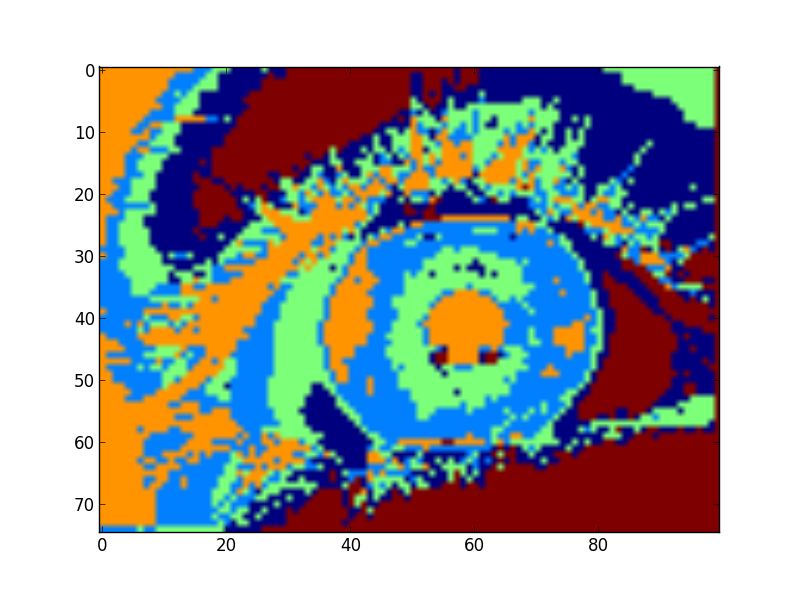
\includegraphics[width=\columnwidth]{Handin1/images/k-means.png}
\caption{k-means clustering}
\label{fig:kmeans}
\end{figure}

Since the pupil is usually very dark, it is (in most cases) safe to assume that it will be contained in the first cluster (the darkest). Therefore k-means can be used in this way to circumvent the need of setting threshold values for the thresholding function that comes next. Instead of a pre-chosen threshold we simply use the value of the first cluster. That ensures that the threshold will be set to contain the darkest values in the image (and by extension likely the pupil). The thresholded image obtained using the k-means from Figure \ref{fig:kmeans} can be seen in Figure \ref{subfig:thresh}. 

\begin{figure}[h!]
	\centering
	
	\begin{subfigure}[b]{0.5\textwidth}
		\centering
		
\includegraphics[width=\textwidth]{Handin1/images/thresh.png}
		\caption{After Thresholding}
		\label{subfig:thresh}
	\end{subfigure}%
	~
	\begin{subfigure}[b]{0.5\textwidth}
		\centering
		
\includegraphics[width=\textwidth]{Handin1/images/open.png}
		\caption{After Opening}
		\label{subfig:open}
	\end{subfigure}
	
	\caption{Thresholding and Opening}
	\label{fig:threshopen}
\end{figure}

After thresholding we perform opening.  Opening is a morphological operation that consists of performing erosion followed by dilation. This cleans up the image, removing noise and speckles. You can see this in the Figure \ref{subfig:open}.

This gives us an image that is well suited for blob analysis. We perform this in two steps. First we remove all blobs which are bigger than 30\% of the image area or smaller than 0.2\% of the entire image. This removes blobs that are most likely not pupil. Second fit an ellipse to the contour and then we compare the ratio between the two radii of that ellipse. That removes all matches that are too elliptical. The pupil is usually more like a circle, but can be slightly elliptical when the user is looking to the side.

The last step we perform is ordering, we order all detected ellipses by increasing extend. This ensures that the most contained blobs come first. In most cases this should prioritize well contained blobs (such as the pupil) over false positives, and all the other detection functions just take the first result from pupil detection.

We have also implemented a failsafe mechanism, that, in absence of any pupils detected, can iteratively call the getPupils() function with lower values of k, which results in better performance in sequences with high contrast. In particular in sequence 8 this change alone has improved the detection rate from 0\% to 62.5\% in the testing frames.

\subsection{Iris Detection}

For iris detection we start with the position of the pupil detected previously. First we filter the image using the Sobel filter. Then we use the filtered image to calculate orientation (Figure \ref{subfig:quiver}) and magnitude (Figure \ref{subfig:magnitude}) of the gradient image. 

\begin{figure}[h!]
	\centering
	
	\begin{subfigure}[b]{0.5\textwidth}
		\centering
		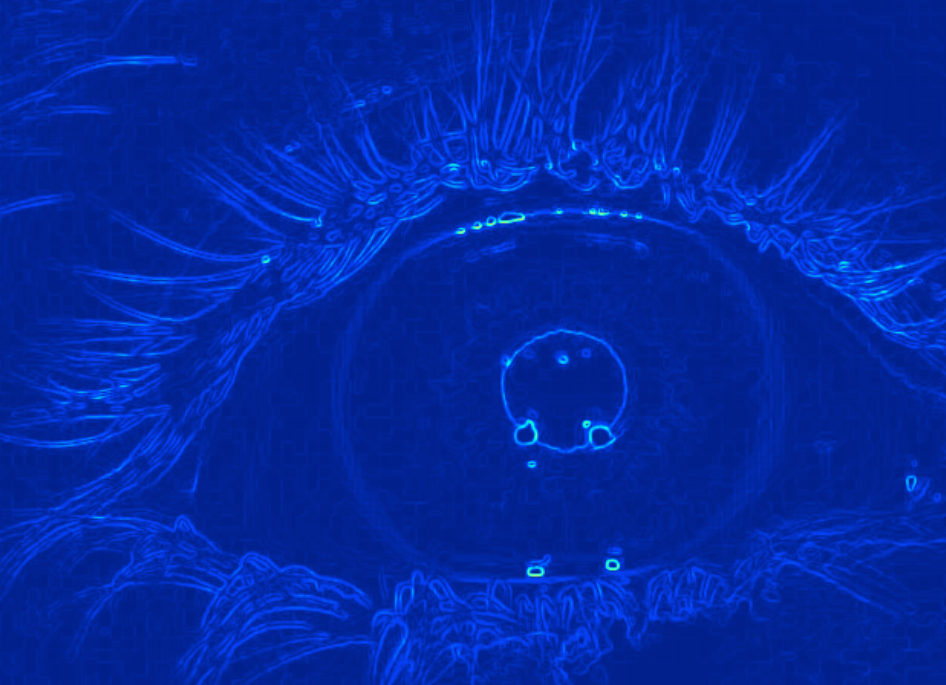
\includegraphics[width=\textwidth]{Handin1/images/magnitude.png}
		\caption{Magnitude}
		\label{subfig:magnitude}
	\end{subfigure}%
	~
	\begin{subfigure}[b]{0.5\textwidth}
		\centering
		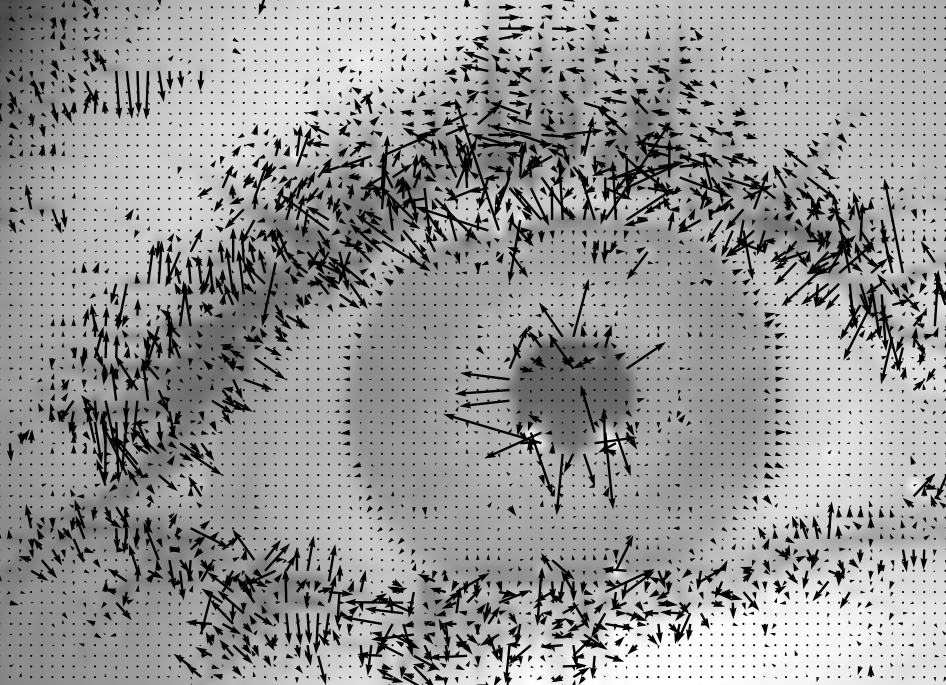
\includegraphics[width=\textwidth]{Handin1/images/quiver.png}
		\caption{Orientation}
		\label{subfig:quiver}
	\end{subfigure}
	
	\caption{Gradient Image: Magnitude and Orientation}
\end{figure}

Then we use the orientation and magnitude data to estimate the iris radius. We assume that the center of iris will be the same as the center of pupil, so we sample the circle defined by pupil on 30 locations and consider lines that originate between the center of the pupil and end at a distance 5x greater than the radius of the pupil. See Figure \ref{subfig:iris_samples} for reference, samples are represented as bright green lines. 
Also in the Figure \ref{subfig:iris_samples} we can see points where sample values for orientation and magnitude correspond to the right values, and therefore are potential candidates for iris boundary. These points are represented as cyan circles in the image. The corresponding magnitude has to be greater than 15 and orientation can be no more than  5 either way from the orientation of the sample line. For each of these points we record the distance from the pupil centre, if more than one point votes for the same radius, we increment the count for that radius. At the end of this process we take the radius with most votes and proclaim it the iris boundary (Shown as a purple circle in Figure \ref{subfig:iris_estimation}).

\begin{figure}[h!]
	\centering
	
	\begin{subfigure}[b]{0.5\textwidth}
		\centering
		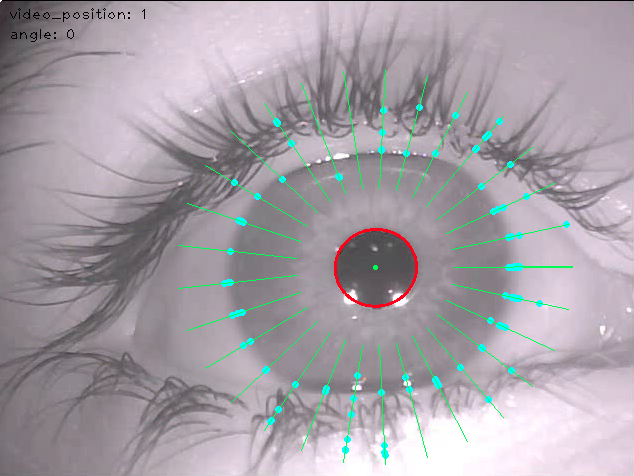
\includegraphics[width=\textwidth]{Handin1/images/iris_samples.png}
		\caption{Samples}
		\label{subfig:iris_samples}
	\end{subfigure}%
	~
	\begin{subfigure}[b]{0.5\textwidth}
		\centering
		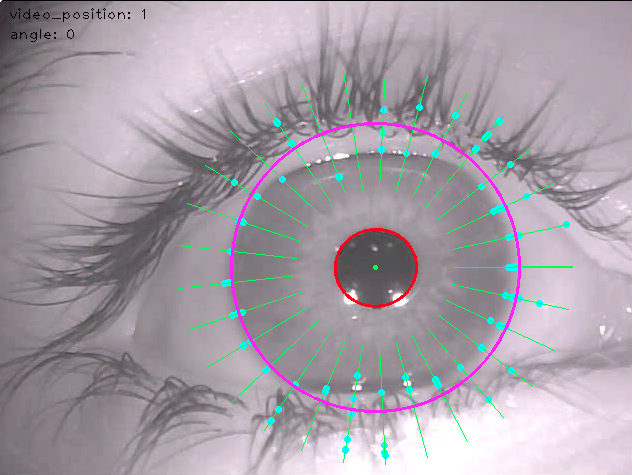
\includegraphics[width=\textwidth]{Handin1/images/iris_estimation.png}
		\caption{Estimation}
		\label{subfig:iris_estimation}
	\end{subfigure}
	
	\caption{Iris Estimation}
\end{figure}

Iris detection works a bit differently than pupil and glint detection in that it works with the assumption that the pupil was detected correctly and therefore there should be an iris to be found. So the detector just counts different votes for individual circle radii and picks the highest one. Of course the worst case for this is when pupil has been mis-detected and there is at least one corresponding orientation and magnitude for one of the 30 sample lines taken, which is highly probable. In this case the iris will be detected on this radius, even though there is only one vote.


\subsection{Glint Detection}

Glint detection is in principle very similar to pupil detection, first we compute k-means to a downsized gray scale image. Since the glint can be considered a flash of light in the eye, we assume that this will the brightest point with the first cluster. 
Therefore, we can use k-means to set the values for the thresholding functions, which are called next. After thresholding we find blobs in the image using contours. We then reject all blobs that are bigger than 0.1\% of the total image area. This ensures that we don't count big bright areas of the image as glints, since glints are usually small. As the last filter we reject all glints that have centers outside of the iris circle which we have calculated in the previous phase. This will leave us only with the glints inside the eye and nothing else.

\begin{figure}[h!]
	\centering
	
	\begin{subfigure}[b]{0.5\textwidth}
		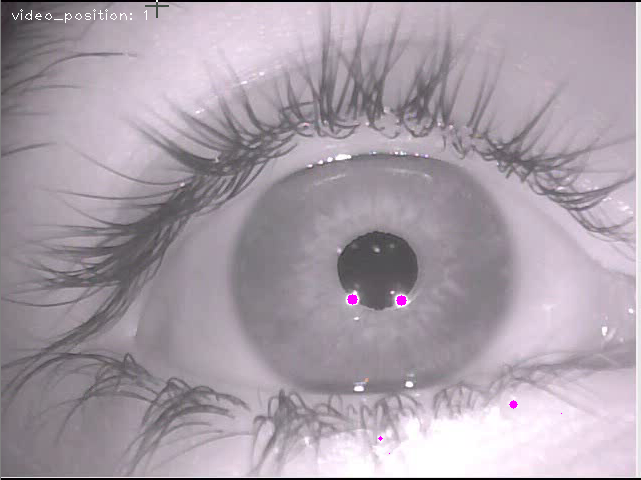
\includegraphics[width=\textwidth]{Handin1/images/glitDetection.png}
		\caption{Glint Detection}
		\label{subfig:glints}
	\end{subfigure}%
	~
	\begin{subfigure}[b]{0.5\textwidth}
		\centering
		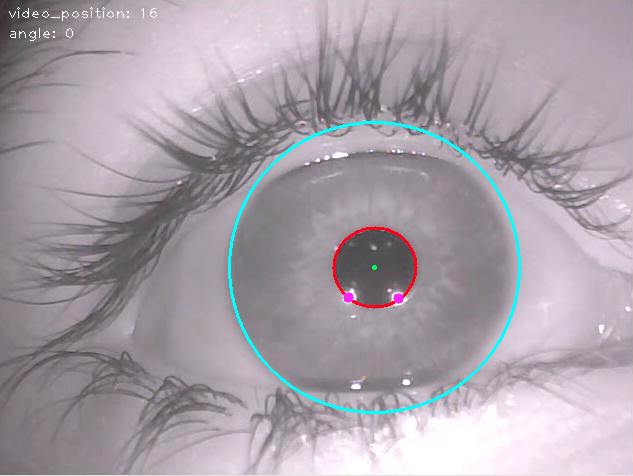
\includegraphics[width=\textwidth]{Handin1/images/final.png}
		\caption{Final Image}
		\label{subfig:final}
	\end{subfigure}
	
	\caption{Glint Detection Phase}
\end{figure}





\section{Results}

In order to test our results, we have built a testing framework. The requirements for this were, that it should allow us to quickly and accurately evaluate changes to the detection algorithms. Manual testing is good, but requires us to manually select a sequence and a frame, which can get tedious very quickly.

To combat this, and also get more consistent results, we have defined an array of representative frames from each sequence. We have carefully selected the frames which we had found to cause most problems for our detection algorithms during manual testing. Therefore our representative sample contains the worst-case frames for each sequence (eye looking different directions, challenging light, or eye position). 

On the other hand, we have selected only 5-8 frames per sequence (56 frames together), so the testing can quickly finish and produce representative results. We have also made sure that all of the frames in question do contain the pupil (i.e no frames with closed eye or where no detection can be made) The testing script also writes all the frames with pupil/iris/glint detections drawn on top into a folder for further (manual) inspection.

Unfortunately we cannot automatically test if a detection is correct, because we have no reference implementation, so the correction still has to be evaluated manually. But what we can detect automatically is the number of detected results (i.e what percentage of images that contained eye have had at least something detected by our implementation). This can at least give us  at least preliminary results, if we assume that most of the detected pupils are correct, we should get a good idea about the results from this alone. Of course this does not mean that we can solely rely on this automatic testing and therefore manual verification still has to be performed.

\begin{table}[h!]
	\center
	\begin{tabular}{ |l|l|l|l| }
		\hline
		Sequence & Frames Evaluated & Pupil Detected & Detected Correctly \\ \hline
		
		eye1.avi 	& 5 	& 5 (100\%)	& 5 (100\%) \\
		eye2.avi 	& 6 	& 6 (100\%)	& 6 (100\%) \\
		eye3.avi 	& 8 	& 8 (100\%)	& 5 (62.5\%) \\
		eye4.avi 	& 8 	& 6 (75\%)	& 6 (75\%) \\
		eye5.avi 	& 6 	& 5 (83.3\%)	& 2 (33.3\%) \\
		eye6.avi 	& 7 	& 7 (100\%)	& 5 (71.43\%) \\
		eye7.avi 	& 8 	& 8 (100\%)	& 8 (100\%) \\
		eye8.avi 	& 8 	& 5 (62.5\%)	& 5 (62.5\%) \\
		
		\hline
		Total 	& 56 & 50 (89.29\%) & 42 (75\%) \\ 
		\hline
	\end{tabular}
	\caption{Semi-Automatic Evaluation of the Detection Algorithm}
	\label{tab:eval}
\end{table}

The Table \ref{tab:eval} shows how many frames were evaluated per sequence, how many of those frames have had something detected by our algorithm (counted automatically during testing) and lastly, how many of the frames have the pupil detected correctly \footnote{By definition of our sample, all frames have the pupil present, so it is an error of the algorithm if it is not detected} (this has been done by manual inspection of all generated frames, i.e pupil detected is right size and corresponds to the actual location of the pupil in the image). 

\begin{figure}[t]
	\centering
	
	\begin{subfigure}[b]{0.5\textwidth}
		\centering
		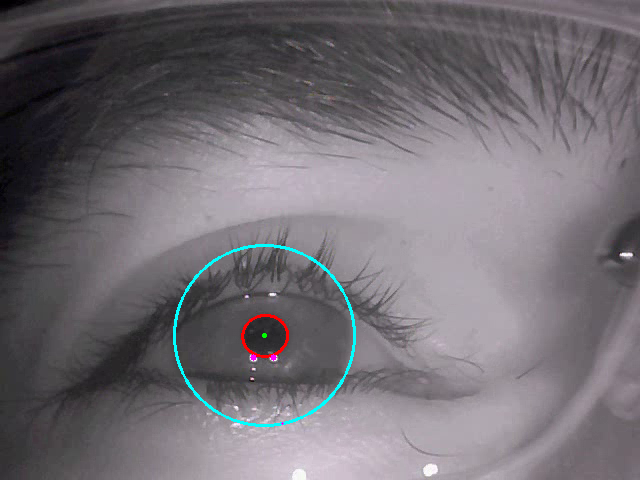
\includegraphics[width=\textwidth]{Handin1/images/good1.png}
		\caption{Eye Squinting}
		\label{subfig:squinting}
	\end{subfigure}%
	~
	\begin{subfigure}[b]{0.5\textwidth}
		\centering
		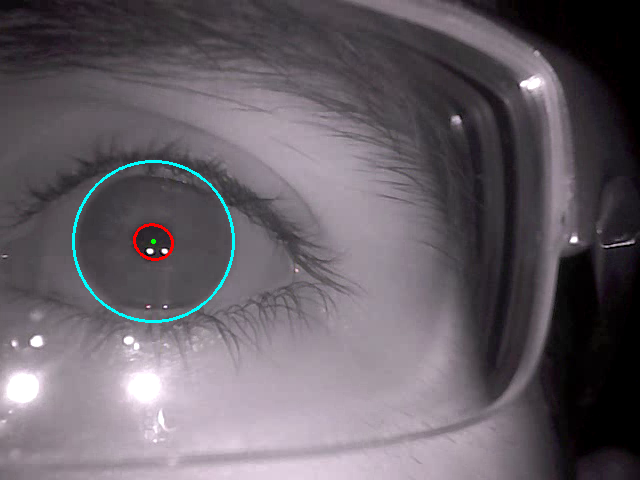
\includegraphics[width=\textwidth]{Handin1/images/good2.png}
		\caption{Challenging Light}
		\label{subfig:challenging_light}
	\end{subfigure}
	
	\begin{subfigure}[b]{0.5\textwidth}
		\centering
		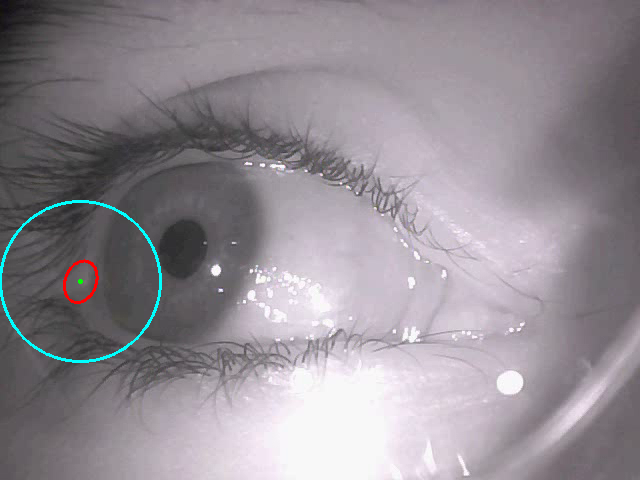
\includegraphics[width=\textwidth]{Handin1/images/wrong1.png}
		\caption{Wrong Detection}
		\label{subfig:wrong1}
	\end{subfigure}%
	~
	\begin{subfigure}[b]{0.5\textwidth}
		\centering
		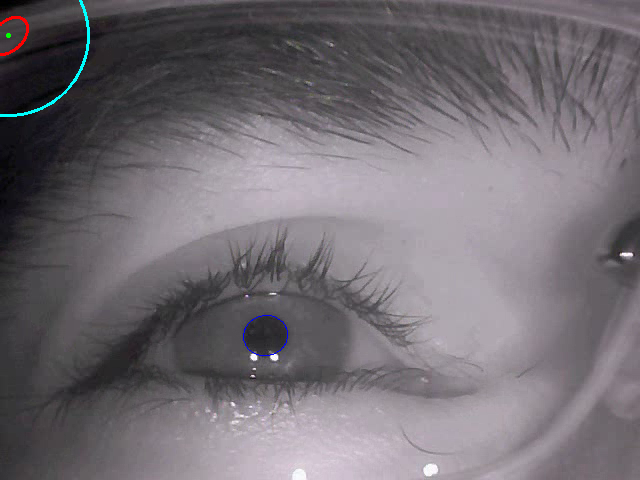
\includegraphics[width=\textwidth]{Handin1/images/wrong2.png}
		\caption{Ordering By Extend}
		\label{subfig:extend}
	\end{subfigure}
	
	\caption{Results}
	\label{fig:results}
\end{figure}

Figure \ref{fig:results} shows good results in the first row (images (a) and (b)) under challenging conditions, as well as wrong results that can occur in row two (images (c) and (d)). In Figure \ref{subfig:extend} you can see a blue circle around the pupil, which is an alternative blob that has been considered by the algorithm, but was most likely rejected because the closing in combination with glints have increased its extend in comparison with the other candidate.

\subsection{Discussion}
In the following text we look at the weaknesses of our algorithm, why it does not work in all frames, and how it could be improved. We look at three interesting points of view from which the work could be improved. First we look at performance, where we evaluate what could be done better to improve performance, second and third we discuss false positives and negatives, which occurred during our testing, what reasons there were for this and how could the algorithm be improved.

\subsubsection{Performance}
Regarding performance, our algorithm is not achieving very good results, primarily because we focused on the detection and code readability, and due to shortage of time we could not work on the speed optimizations as we would have liked. However we can mention some of the sacrifices we have made to improve code readability and ease of handling during testing. 
For example in various parts of the algorithm we use the gray scale image, which we most of the time just calculate again, instead we could either implement some sort of cache or pass the gray scale image around and only generate it once. Similar story is with k-means image. We use the same algorithm in pupil and glint detection, yet these two don’t share the results, which they should.

\subsubsection{False Positives}
False positives are cases where a pupil is detected in a place where it is not actually supposed to be. We have found that this usually occurs when there are very dark areas in the image. This confuses the k-means, producing the darkest region that does not necessarily contain the pupil, at which point the whole algorithm is destined to fail. It will pick a blob that best resembles the pupil out of those available and try to work with that, producing wrong results. 
A solution we have tried to combat this problem is overlaying a transparent-to-white radial gradient from the center of the image to suppress the dark areas around image edges. But what we found was that even though the number of detections in sequences that were most affected by the above described problem went up, the overall results over all of the sequences were worse. So we decided against that improvement. However it still might be warranted to selectively apply it to only some of the sequences, if it can be safely assumed that the pupil stays near the center of the frame and there are dark areas near the edges of the frame.

\subsubsection{False Negatives}
False negatives are produced when a pupil should have been detected, but was not. These cases can be caught by our automated testing, because all of the frames being tested should contain a pupil. This is of course very similar to the previous case with k-means, but we have to manage limiting this problem using the iterative lowering of k-means parameter.

\include{Handin1/further_work}
\section{Conclusion}


%%% End document
\end{document}